\begin{figure}
  \setlength{\unitlength}{\textwidth}
\fbox{
  \begin{picture}(0.95,1.3)(0,0.7)
    % % %90
      % % % Parkinson Data 
      \put(0.035,1.65){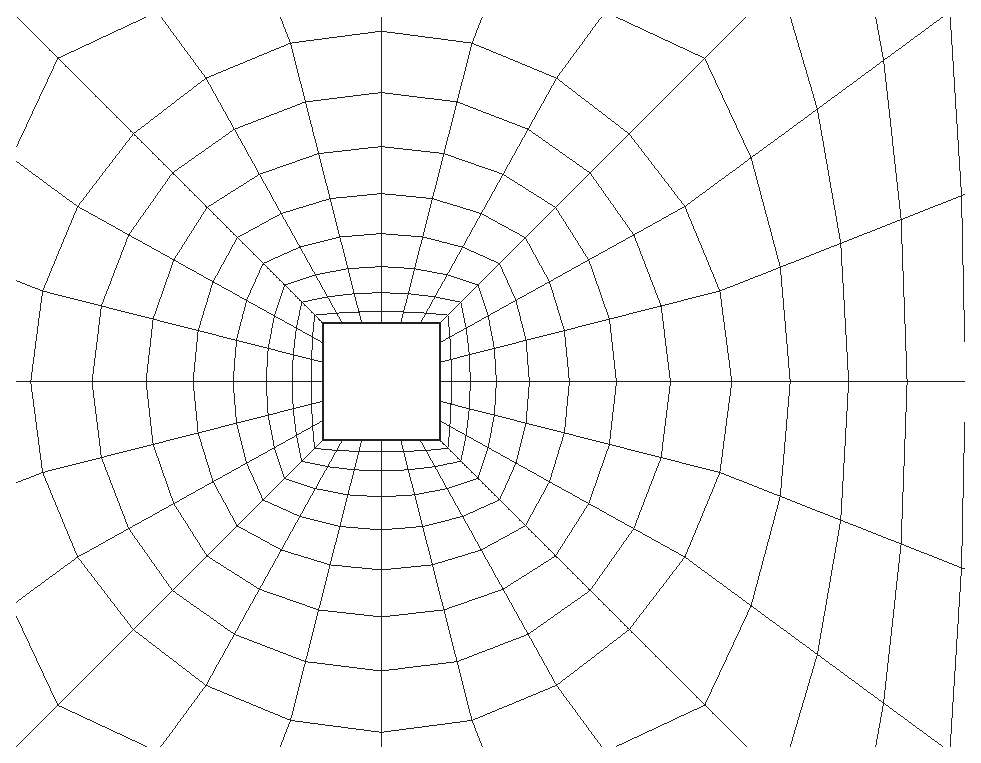
\includegraphics[width=0.4\unitlength]{./chapter-methodology/fnp/mesh.eps}}
      \put(0.495,1.65){\includegraphics[width=0.4\unitlength]{./chapter-methodology/fnp/{hyb0.75-mesh}.eps}}
      \put(0.035,1.25){\includegraphics[width=0.4\unitlength]{./chapter-methodology/fnp/{hyb0.5-mesh}.eps}}
      \put(0.495,1.25){\includegraphics[width=0.4\unitlength]{./chapter-methodology/fnp/{hyb0.25-mesh}.eps}}
      \put(0.3,0.85){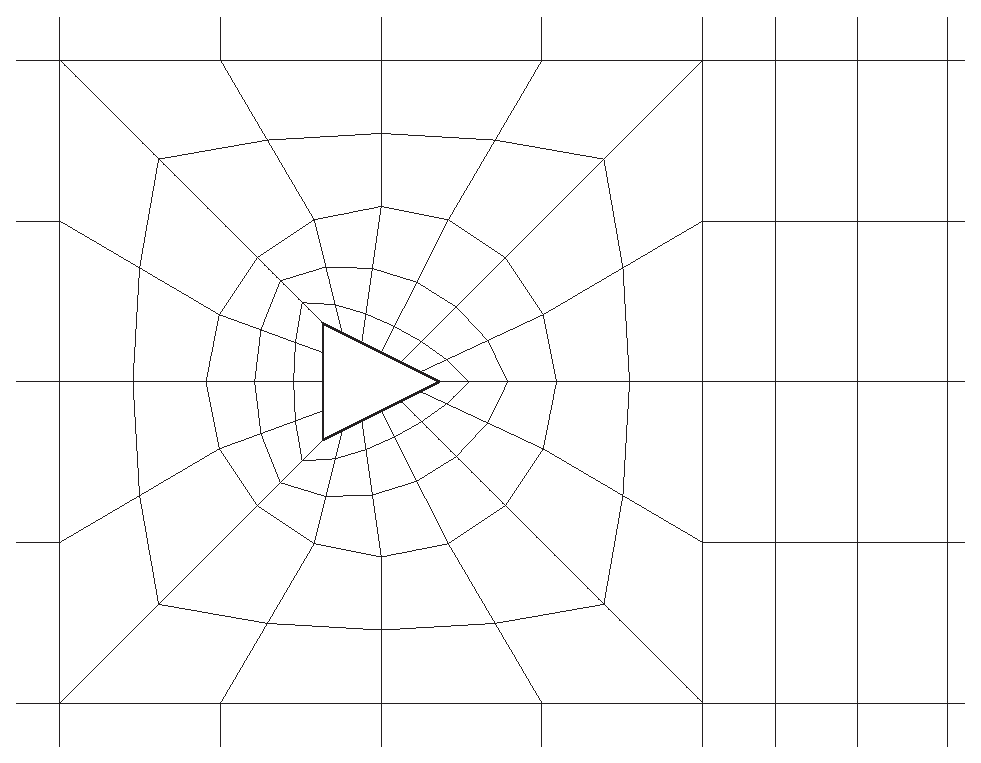
\includegraphics[width=0.4\unitlength]{./chapter-methodology/fnp/triangle-mesh.eps}}
      
      
   
      
      
%      \put(0.23,0.00){ $\displaystyle\frac{c}{\rho\mathcal{A}U}$}
%      \put(0.73,0.00){ $\displaystyle\frac{c}{\rho\mathcal{A}U}$}

     
      \put(0.206,1.605){\small(a)}
      \put(0.665,1.605){\small(b)}
      \put(0.206,1.2){\small(c)}
      \put(0.665,1.2){\small(d)}
      \put(0.45,0.8){\small(e)}
      

  \end{picture}
}
\caption{Configuration of the macro elements near the cross section. (a) square, (b) $\ratio=0.75$, (c) $\ratio=0.5$, (d) $\ratio=0.25$ and (e) triangle.}
  
  \label{fig:zoom-mesh}
\end{figure}